\begin{figure}[h!]
	\centering
	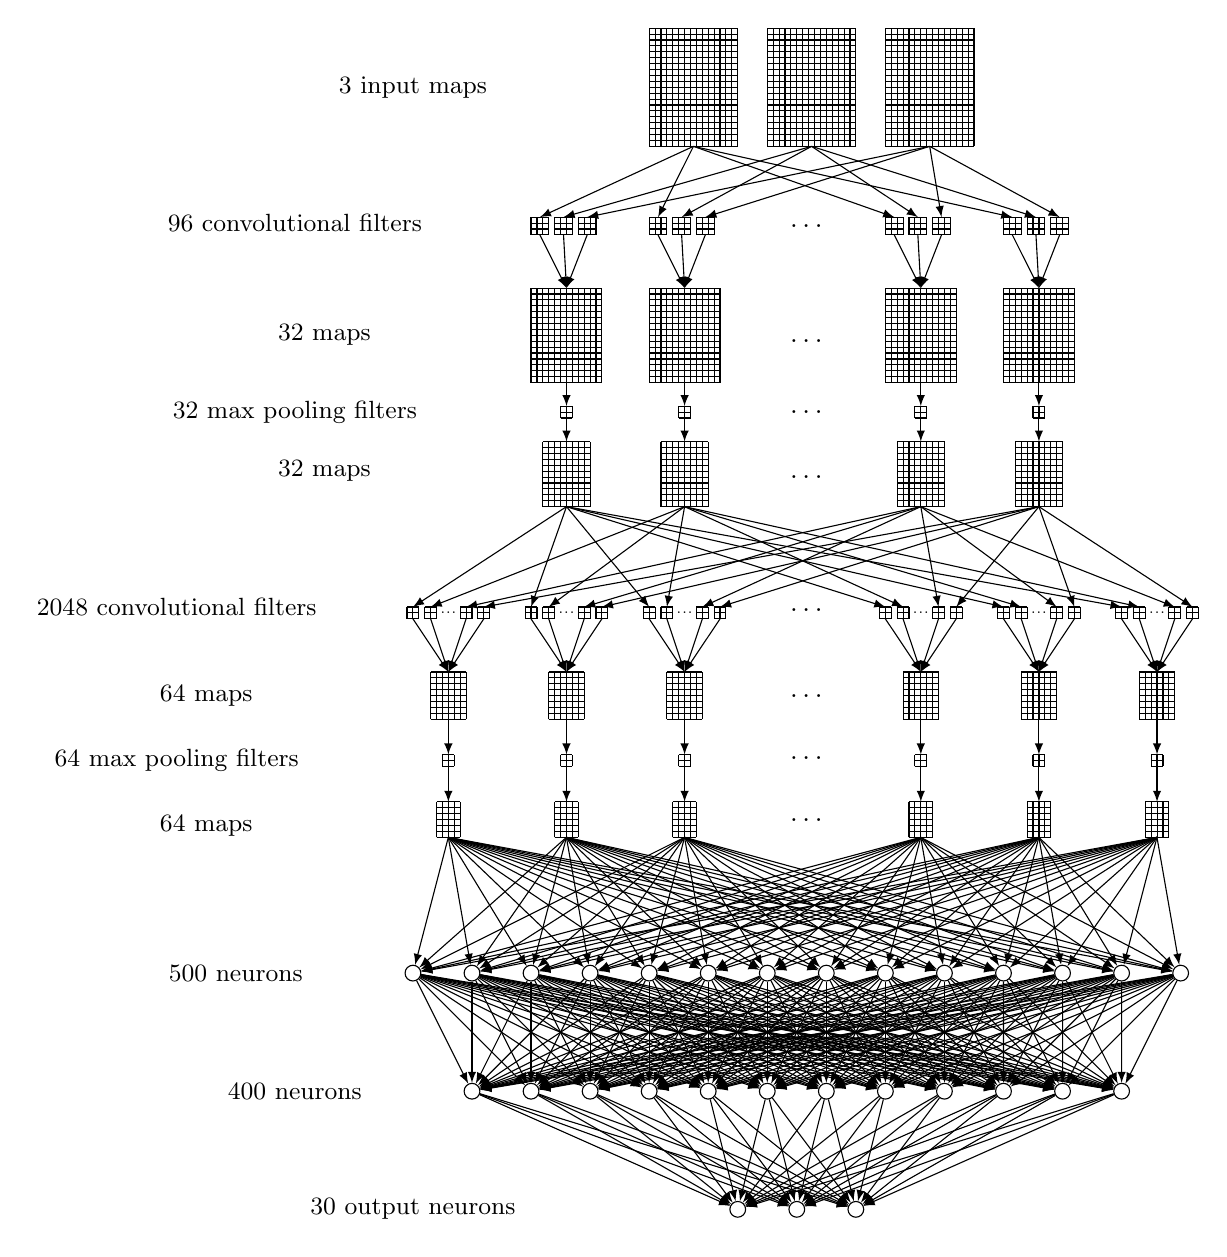
\begin{tikzpicture}[scale=0.75,every path/.style={>=latex}]%0.635%0.73
		% ========================================================================================= %
		% draw input maps
		\def\limX{0} % x-position of the leftmost input map
		\def\limY{1} % y-position of the leftmost input map
		\node at (\limX - 4, \limY + 1) {\small 3 input maps};
		
		\draw[step=0.1] (\limX,\limY) grid (\limX + 1.5,\limY + 2.0);
		\draw[step=0.1] (\limX + 2,\limY) grid (\limX + 3.5,\limY + 2.0);
		\draw[step=0.1] (\limX + 4,\limY) grid (\limX + 5.5,\limY + 2.0);
		
		% ========================================================================================= %
		% draw first convolutional and max pooling layer
		\def\lflmX{-5} % x-position of the leftmost first layer map
		\def\lflmY{-3} % y-position of the leftmost first layer map
		\node at (\lflmX - 1, \lflmY + 2.7) {\small 96 convolutional filters};
		\node at (\lflmX - 0.5, \lflmY + 0.8) {\small 32 maps};
		\node at (\lflmX - 1, \lflmY - 0.5) {\small 32 max pooling filters};
		\node at (\lflmX - 0.5, \lflmY - 1.5) {\small 32 maps};
		
		\foreach \x in {-1,0,2,3}
		{
			% draw maps of the first convolutional layer
			\draw[step=0.1] (2 * \x - 0.001,\lflmY - 0.001) grid (2* \x + 1.201,\lflmY + 1.6);
			
			% draw filters to the map
			\foreach \i in {0,...,2}
			{
				% draw filter
				\draw[step=0.1] (2 * \x + 0.4 * \i - 0.001,\lflmY + 2.5 - 0.001) grid (2* \x + 0.4 * \i + .301,\lflmY + 2.5 + .301);
				
				% draw connections from input maps to the filters
				\draw[->] (\limX + \i * 2 + 0.75,\limY) to (2 * \x + 0.4 * \i + 0.15,\lflmY + 2.5 + .301);
				
				% draw connections from filter to next map
				\draw[->] (2 * \x + 0.4 * \i + 0.15, \lflmY + 2.5 - 0.001) to (2 * \x + 0.6,\lflmY + 1.6);
			}
		
			% draw max pooling filter
			\draw[step=0.1] (2 * \x + 0.499,\lflmY - .601) grid (2* \x + .701,\lflmY - .399);
			
			% draw connection from first convolutional layer maps to max pooling filters
			\draw[->] (2* \x + 0.6,\lflmY + 1.6) to (2* \x + .6,\lflmY - .399);
			
			% draw first max pooling layer map
			\draw[step=0.1] (2 * \x + 0.199,\lflmY - 2.101) grid (2* \x + 1.001,\lflmY + -1.0);
			
			% draw connection from max pooling filter to max pooling map
			\draw[->] (2 * \x + 0.6,\lflmY - .601) to (2* \x + .6,\lflmY + -1.0);
		}
		
		% draw dots between the filters and the first layer maps
		\node at (\lflmX + 7.7, \lflmY - 1.6) {\ldots};
		\node at (\lflmX + 7.7, \lflmY - 0.5) {\ldots};
		\node at (\lflmX + 7.7, \lflmY + 0.7) {\ldots};
		\node at (\lflmX + 7.7, \lflmY + 2.65) {\ldots};
		
		% ========================================================================================= %
		% draw second convolutional and max pooling layer
		\def\lslmX{-5} % x-position of the leftmost first layer map
		\def\lslmY{-9.5} % y-position of the leftmost first layer map

		\node at (\lslmX - 3, \lslmY + 2.7) {\small 2048 convolutional filters};
		\node at (\lslmX - 2.5, \lslmY + 1.2) {\small 64 maps};
		\node at (\lslmX - 3, \lslmY + 0.1) {\small 64 max pooling filters};
		\node at (\lslmX - 2.5, \lslmY - 1.0) {\small 64 maps};
		
		\foreach \x in {-2,-1,0,2,3,4}
		{
			% draw second convolutional layer maps
			\draw[step=0.1] (2 * \x + 0.299,\lslmY + 0.799) grid (2* \x + 0.901,\lslmY + 1.6);
			
			% draw filters to the map
			\foreach \i in {-1,0,2,3}
			{
				% draw filter
				\draw[step=0.1] (2 * \x + 0.3 * \i + 0.199,\lslmY + 2.5 - 0.001) grid (2* \x + 0.3 * \i + .401,\lslmY + 2.5 + .201);
				
				% draw connections from first max pooling layer maps to the filters
				\draw[->] (2 * \i + 0.6,\lflmY - 2.101) to (2* \x + 0.3 * \i + .3,\lslmY + 2.4 + .301);
				
				% draw connections from filter to next map
				\draw[->] (2 * \x + 0.3 * \i + 0.3, \lslmY + 2.5 - 0.001) to (2 * \x + 0.6,\lslmY + 1.6);
			}
			
			% draw dots between the filters of this map
			\node at (2 * \x + 0.6,\lslmY + 2.6) {\tiny ...};
			
			% draw max pooling filter
			\draw[step=0.1] (2 * \x + 0.499,\lslmY - .001) grid (2* \x + .701,\lslmY + .201);
			
			% draw connection from second convolutional layer maps to max pooling filters
			\draw[->] (2* \x + 0.6,\lslmY + 1.6) to (2* \x + .6,\lslmY + .201);
			
			% draw second max pooling layer map
			\draw[step=0.1] (2 * \x + 0.399,\lslmY - 1.201) grid (2* \x + .801,\lslmY + -0.6);
			
			% draw connection from max pooling filter to max pooling map
			\draw[->] (2 * \x + 0.6,\lslmY + .201) to (2* \x + .6,\lslmY + -0.6);
		}
		
		% draw dots between the filters and the first layer maps
		\node at (\lslmX + 7.7, \lslmY + 0.15) {\ldots};
		\node at (\lslmX + 7.7, \lslmY - 0.9) {\ldots};
		\node at (\lslmX + 7.7, \lslmY + 1.2) {\ldots};
		\node at (\lslmX + 7.7, \lslmY + 2.65) {\ldots};
		
		% ========================================================================================= %
		% draw first fully connected layer
		\def\lffclX{-4} % leftmost x-position of the first fully connected layer
		\def\rffclX{9} % rightmost x-position of the first fully connected layer
		\def\ffclY{-13} % y-position of the first fully connected layer
		\node at (\lffclX - 3,\ffclY) {\small 500 neurons};
		
		\foreach \x in {\lffclX,...,\rffclX}
		{
			\node (n\x) at (\x,\ffclY) [draw,circle,inner sep=0pt,minimum size = 0.2cm] {};
			
			\foreach \a in {-2,-1,0,2,3,4}
			{
				\draw[->] (2 * \a + 0.599,\lslmY - 1.201) to (n\x);
			}
		}
		
		% ========================================================================================= %
		% draw second fully connected layer
		\def\lsfclX{-3} % leftmost x-position of the second fully connected layer
		\def\rsfclX{8} % rightmost x-position of the second fully connected layer
		\def\sfclY{-15.} % y-position of the second fully connected layer
		\node at (\lsfclX - 3,\sfclY) {\small 400 neurons};
		
		\foreach \x in {\lsfclX,...,\rsfclX}
		{
			\node (m\x) at (\x,\sfclY) [draw,circle,inner sep=0pt,minimum size = 0.2cm] {};
			
			\foreach \a in {\lffclX,...,\rffclX}
			{
				\draw[->] (n\a) to (m\x);
			}
		}
		
		% ========================================================================================= %
		% draw output layer
		\def\lolX{1} % leftmost x-position of the output layer
		\def\rolX{3} % rightmost x-position of the output layer
		\def\olY{-17.} % y-position of the output layer
		\node at (\lolX - 5,\olY) {\small 30 output neurons};
		
		\foreach \x in {\lolX,...,\rolX}
		{
			\node (q\x) at (\x + 0.5,\olY) [draw,circle,inner sep=0pt,minimum size = 0.2cm] {};
			
			\foreach \a in {\lsfclX,...,\rsfclX}
			{
				\draw[->] (m\a) to (q\x);
			}
		}
	\end{tikzpicture}
	\caption{A complete example \ac{CNN}}
	\label{fig:example_cnn}
\end{figure}
